\documentclass{article}
\usepackage{listings}
\usepackage[]{hyperref}
\hypersetup{colorlinks=true,}
\usepackage{graphicx} % Required for inserting images
\usepackage{multirow}
\usepackage{tfrupee}
\usepackage{geometry}
\usepackage{subcaption}
\geometry{a4paper, portrait, margin=1in}




\begin{document}


\begin{titlepage}
    	
    	\begin{center}
		\begin{LARGE}
		\bf{Facial Recognition on an FPGA\\}
		\end{LARGE}
		\vspace{40pt}
		
		\vspace{6pt}
		\textbf{\Large EE 396}\\
		\vspace{6pt}
		\textbf{\Large Design Laboratory}\\
		\vspace{40pt}
		
		\textbf{\Large
			Yash Kataria : 210102100\\
			Lakshit Sethia : 210102123\\}
		\vspace{60pt}
		
\includegraphics[width=0.3\textwidth]{IITG_logo.png} \\
		\vspace{60pt}
		\textit{\large Under the supervision of}\\
            \vspace{2mm}
		\textbf{\Large Prof. Gaurav Trivedi }\\
            \vspace{4mm}
            \textit{\large Guided by} \\
            \vspace{2mm}
            \textbf{\Large Saras Mani Mishra}
		
		
		\vspace{60pt}
		
		
		\textbf{\large EEE Department\\
			Indian Institute of Technology, Guwahati\\
			\today
		}
	\end{center}

\end{titlepage}



\newpage
\section*{Abstract}
\large 
The utilization of Field-Programmable Gate Arrays (FPGAs) has garnered significant attention in recent years due to their capacity to enhance performance in neural network models by enabling parallel processing of data. This project explores the integration of FPGA technology to bolster the efficacy of convolutional neural network (CNN) models, specifically focusing on the ResNet-18 architecture. Facial recognition emerges as a pertinent domain where the amalgamation of machine learning expertise holds promise for addressing real-world challenges, particularly in security and attendance systems. Leveraging FPGA-based acceleration, our endeavor aims to not only refine the efficiency and speed of CNN computations but also to furnish practical solutions for facial recognition tasks. Through the implementation of ResNet-18 on FPGA, this project endeavors to contribute to the advancement of facial recognition technologies with tangible applications in security and attendance systems.
\newpage

{ \hypersetup{linkcolor=blue} \tableofcontents }

\newpage

\section{Introduction}
Our journey of building this project has led to an in-depth exploration of various machine learning techniques and models.
\\
\\Initially, Principal Component Analysis (PCA) was explored as a method for feature extraction and dimensionality reduction. While PCA offered simplicity in implementation, its effectiveness was limited, resulting in subpar accuracy for our recognition task.
\\
\\To overcome these limitations, we progressed to leverage Deep Learning architectures, primarily Convolution Neural Networks(CNNs) to perform our task.
\\
\\Subsequently, we adopted the ResNet-18 architecture, which strikes a balance between computational efficiency and accuracy. The inherent efficiency of ResNet-18 aligns well with the resource constraints of FPGA, enabling accelerated inference without compromising accuracy.
\\
\\Then we progressed to the Verilog implementation, starting implementing layer-by-layer. We had extracted weights and feature vector from the python and done the final execution of fully connected layer and classification on the FPGA. We implemented UART for the data transfer. 
\\
\\The final project was complete with GUI in python to select and upload photo to the FPGA and we could see the output on the FPGA via the LEDs.

\section{Theory}

\subsection{First Approach - Principal Component Analysis}

In face recognition, images of faces are typically high-dimensional data, with each pixel representing a feature. These high-dimensional data can be computationally expensive to work with and may lead to overfitting. Principal Component Analysis (PCA) helps reduce the dimensionality of the data by transforming it into a lower-dimensional space while retaining as much variance as possible. This reduction in dimensionality simplifies subsequent processing steps and improves computational efficiency.

\begin{enumerate}
    \item \textbf{Mean Centering: } Mean centering helps remove spurious correlations in the data. When you compute the covariance matrix or correlation matrix to perform PCA, the presence of the mean value in each feature can lead to misleading correlations. By centering the data, you ensure that the origin of the coordinate system corresponds to the mean of the data, which helps in capturing the true relationships between variables. Also, it allows us to use the Covariance Matrix trick mentioned later.

    \item \textbf{Explained Variance: } Explained variance in Principal Component Analysis (PCA) represents the proportion of the total variance in a dataset that is accounted for by each principal component (PC). In PCA, data is transformed into a new set of orthogonal variables (principal components) that are linear combinations of the original features. These principal components are ordered by the amount of variance they explain, with the first PC explaining the most variance, the second PC explaining the second most, and so on. These variances are proportional to the eigenvalues.

The explained variance of a principal component tells us how much of the variability in the data is captured by that component. It's typically expressed as a percentage, and you can calculate it by dividing the variance of a specific PC by the total variance of the original data. Understanding the explained variance is crucial for dimensionality reduction and selecting the appropriate number of principal components to retain, as it helps you assess how much information is retained while reducing the dimensionality of the data.

\item \textbf{Projection: }
\begin{itemize}
    \item In PCA, projection refers to the process of transforming high-dimensional data (such as images represented as pixel values) onto a lower-dimensional subspace defined by its principal components.

    \item The principal components are orthogonal vectors that capture the directions of maximum variance in the original data. By projecting the data onto these components, you obtain a set of coefficients that represent the contribution of each component to the original data.

    \item In image PCA, projecting an image onto the principal components results in a compressed representation of the image using fewer components. This reduces the dimensionality while retaining the most significant information.
\end{itemize}

\item \textbf{Reconstruction: }
\begin {itemize}
    \item Reconstruction is the process of taking the lower-dimensional representation (obtained through projection) and mapping it back to the original high-dimensional space.

    \item To reconstruct an image from its lower-dimensional representation, you multiply the coefficients obtained during projection by the corresponding principal components and add them together. This process recreates an approximation of the original image.

    \item The quality of the reconstruction depends on the number of principal components used. More components lead to a more faithful representation, while fewer components result in a loss of detail.
    
\end {itemize}

\end{enumerate}

In summary, PCA allows you to reduce the dimensionality of images by projecting them onto a lower-dimensional subspace defined by principal components. You can then reconstruct an approximation of the original image from this reduced representation.

\subsection{Second Approach - ResNet-18}
\begin{enumerate}
    \item \textbf{About the Model: }ResNet-18 is a Convolutional Neural Network (CNN) architecture that belongs to the family of Residual Networks (ResNets), which was introduced by Microsoft Research in their paper "Deep Residual Learning for Image Recognition" in 2015. ResNets are known for their remarkable performance in image recognition tasks, especially in handling the vanishing gradient problem that often hampers the training of very deep neural networks.

    \item \textbf{Architecture of the Model:} Following image depicts the architecture of the ResNet-18 Model.

    \begin{figure}[!hbt]
        \noindent\makebox[\textwidth]{%
        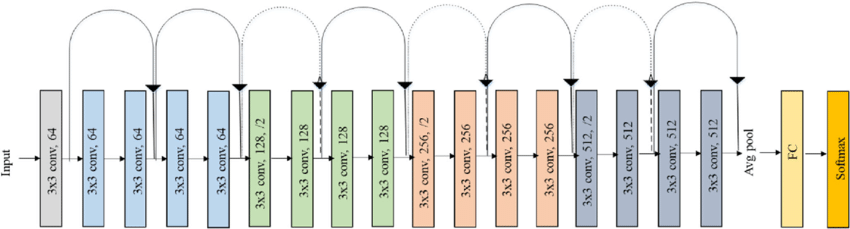
\includegraphics[width=0.9\textwidth]{ResNet-18-Architecture.png}}
        \caption{Architecture of the ResNet-18 Model}
    \end{figure}
    
    It's various components are explained as follows - 
    \begin{itemize}
        \item \textbf{Input:} The network takes an input image with dimensions 224x224x3, where 3 represents the three color channels (red, green, blue).

        \item \textbf{Convolutional Layers:} The network starts with several convolutional layers. Each convolutional layer is represented by a rectangular box, indicating the number of filters (channels) and their spatial dimensions. For example, "3x3 conv 64" denotes a convolutional layer with 64 filters of size 3x3.

        \item \textbf{Max Pooling:} After some convolutional layers, max-pooling layers are applied to reduce the spatial dimensions of the feature maps while retaining important features. Max-pooling is represented by downward arrows.

        \item \textbf{Residual Blocks:} The distinctive feature of ResNet is the use of residual blocks. Each block consists of multiple convolutional layers with skip connections (shortcut connections) that bypass one or more layers. These skip connections help in alleviating the vanishing gradient problem during training, allowing for the successful training of very deep networks.

        \item \textbf{Average Pooling:} At the end of the network, global average pooling is applied to reduce the spatial dimensions of the feature maps to a 1x1 size. This operation computes the average value of each feature map, resulting in a fixed-size representation regardless of the input image size.

        \item \textbf{Fully Connected Layers (FC):} Following the average pooling layer, one or more fully connected layers are used for the final classification. These layers typically have a large number of neurons and serve to map the features learned by the convolutional layers to the output classes.   
        
        \item \textbf{Softmax:} The final layer applies the softmax function, which converts the raw output scores of the network into probabilities. These probabilities represent the likelihood of each class, and the class with the highest probability is predicted as the final output.
    \end{itemize}

    \item \textbf{Advantages of the ResNet-18 for Face Recognition:}

    \begin{itemize}
        \item \textbf{Depth:} ResNet-18 has a moderate depth, which strikes a balance between depth and complexity. It's deep enough to capture intricate features in facial images but not excessively deep to cause overfitting or computational inefficiency.

        \item \textbf{Residual Blocks:} The use of residual blocks allows for effective training of deeper networks without the vanishing gradient problem. This is crucial for face recognition tasks, where the model needs to capture subtle variations in facial features.

        \item \textbf{Transfer Learning:} Pre-trained ResNet-18 models on large-scale image datasets like ImageNet are readily available. These pre-trained models can be fine-tuned on face datasets with relatively small modifications, saving significant computational resources and time.

        \item \textbf{Efficiency:} ResNet-18 strikes a good balance between accuracy and computational efficiency. It's less computationally expensive compared to deeper ResNet variants like ResNet-50 or ResNet-101, making it feasible for deployment on resource-constrained devices like FPGA or in real-time applications.
    \end{itemize}    
\end{enumerate}

\subsection{IEEE Standard 754 Floating Point Numbers}

We had to use the IEEE 754 format in our project as all the parameters of our model were 32-bit floating point numbers. Let's understand what it is. The IEEE Standard for Floating-Point Arithmetic (IEEE 754) is a technical standard for floating-point computation which was established in 1985 by the Institute of Electrical and Electronics Engineers (IEEE). The standard addressed many problems found in the diverse floating point implementations that made them difficult to use reliably and reduced their portability. IEEE Standard 754 floating point is the most common representation today for real numbers on computers, including Intel-based PC’s, Macs, and most Unix platforms.

There are several ways to represent floating point number but IEEE 754 is the most efficient in most cases. IEEE 754 has 3 basic components:

\begin{itemize}
    \item \textbf{The Sign of Mantissa - }This is as simple as the name. 0 represents a positive number while 1 represents a negative number.

    \item \textbf{The Biased Exponent - }The exponent field needs to represent both positive and negative exponents. A bias is added to the actual exponent in order to get the stored exponent.

    \item \textbf{The Normalised Mantissa –}The mantissa is part of a number in scientific notation or a floating-point number, consisting of its significant digits. Here we have only 2 digits, i.e. O and 1. So a normalised mantissa is one with only one 1 to the left of the decimal.
\end{itemize}

\begin{figure}[!hbt]
        \noindent\makebox[\textwidth]{%
        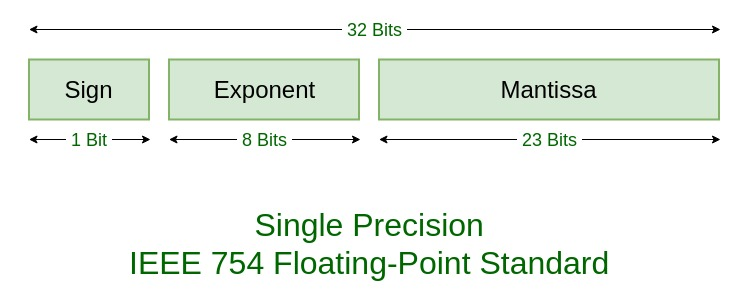
\includegraphics[width=0.9\textwidth]{IEEE-754.jpg}}
        \caption{}
    \end{figure}
    
\section{Development Setup and Components}
     \large 
     \begin{enumerate}
        \item \textbf{Hardware:}
            \begin{itemize}
                \item Nexys A7100T FPGA Board
                \item USB to micro-USB cable
            \end{itemize}
     
         \item \textbf{Softwares:}
         \begin{itemize}
             \item Vivado 2023.2
             \item Visual Studio Code IDE
         \end{itemize}

         \item \textbf{Languages:}
         \begin{itemize}
             \item Verilog
             \item Python (Jupyter Notebook)
         \end{itemize}
     \end{enumerate}
    
\section{Software Implementaion}
\subsection{Tools and Software Used}
\begin{itemize}
\item Visual Studio code for running Jupyter Notebooks
\item NVIDIA's CUDA for faster training times
\item \textbf{Libraries}: Pytorch, OpenCV2, Pandas, Numpy, Matplotlib, Pyserial
\item Vivado 2023.2 for Verilog.
\end{itemize}



% \vspace{0.3in}

    \subsection{Dataset}

    The dataset on which we are training and testing our model is taken from Kaggle - it is the \href{https://www.kaggle.com/dansbecker/5-celebrity-faces-dataset}{\textbf{5 Celebrity Faces Dataset}}.
\\\\
    This is a small dataset for experimenting with computer vision techniques. It has a training directory containing 14-20 photos each of the celebrities - 

    \begin{itemize}
        \item Ben Afflek 
        \item Elton John 
        \item Jerry Seinfeld 
        \item Madonna 
        \item Mindy Kaling 
    \end{itemize}  
    
    The validation directory has 5 photos of each celebrity.
    \begin{figure}[!hbt]
        \noindent\makebox[\textwidth]{%
        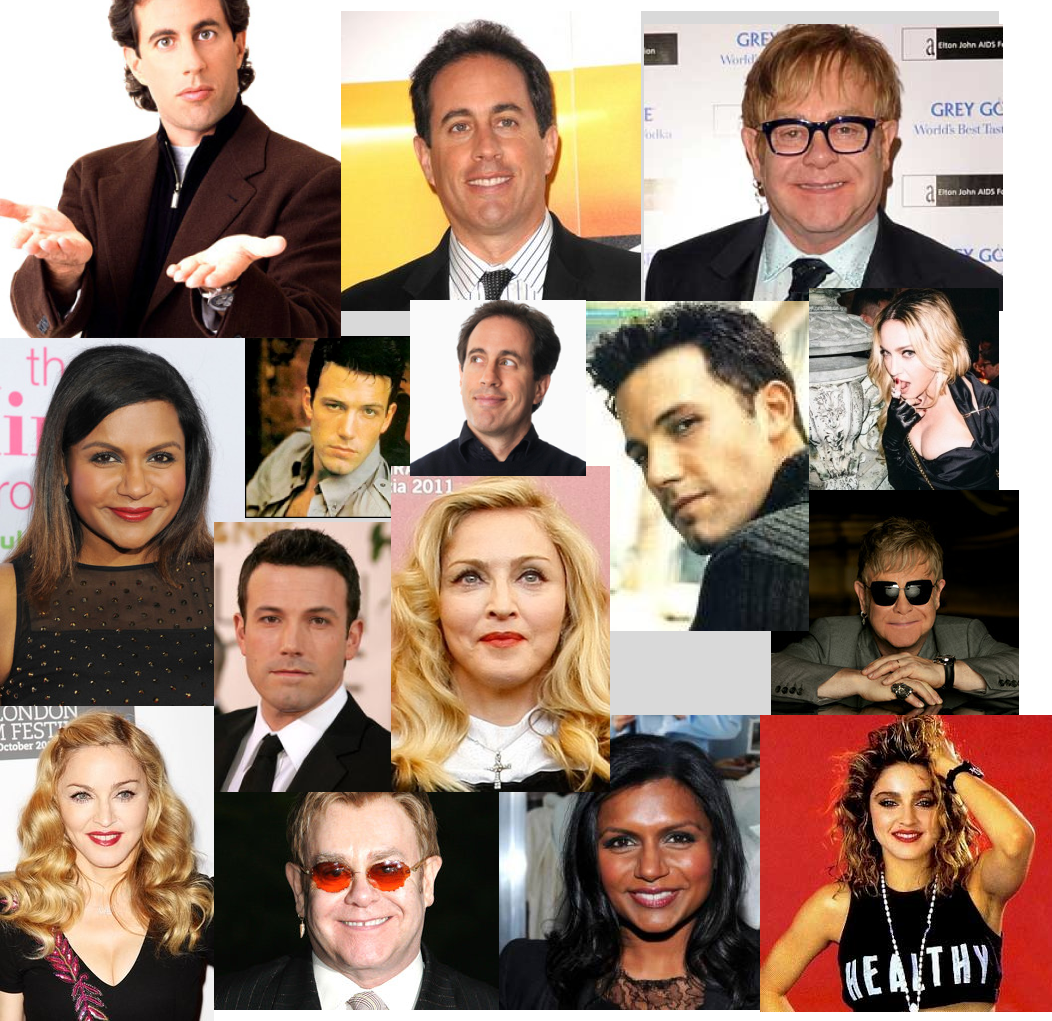
\includegraphics [height = 5cm]  {dataset.png}}
        \caption{Data-set.}
    \end{figure}

    \subsection{Data Preprocessing (Common to both approaches) }

    Haar Cascade was employed for face detection and cropping. Initially, we trained the Haar Cascade classifier using a dataset containing positive and negative images. Positive images depicted faces, while negative images did not. During training, the classifier learned to distinguish facial features by analyzing contrast differences using Haar-like features.
\\
    Once trained, the Haar Cascade classifier was applied to input images for face detection. It scanned the images using a sliding window approach, evaluating regions for facial features based on learned patterns. When a match was found, a bounding box was generated around the detected face.
\\
    After face detection, the bounding box coordinates were used to crop the original image and extract the detected faces. This process involved retaining only the regions within the bounding boxes and discarding the rest of the image.
\\
    Overall, Haar Cascade-based face detection and cropping provided an efficient solution for automatically identifying faces in images. While it offered high accuracy in controlled environments, it might have struggled with challenges such as occlusions and poor lighting conditions.

      \begin{figure}[!hbt]
        \noindent\makebox[\textwidth]{%
        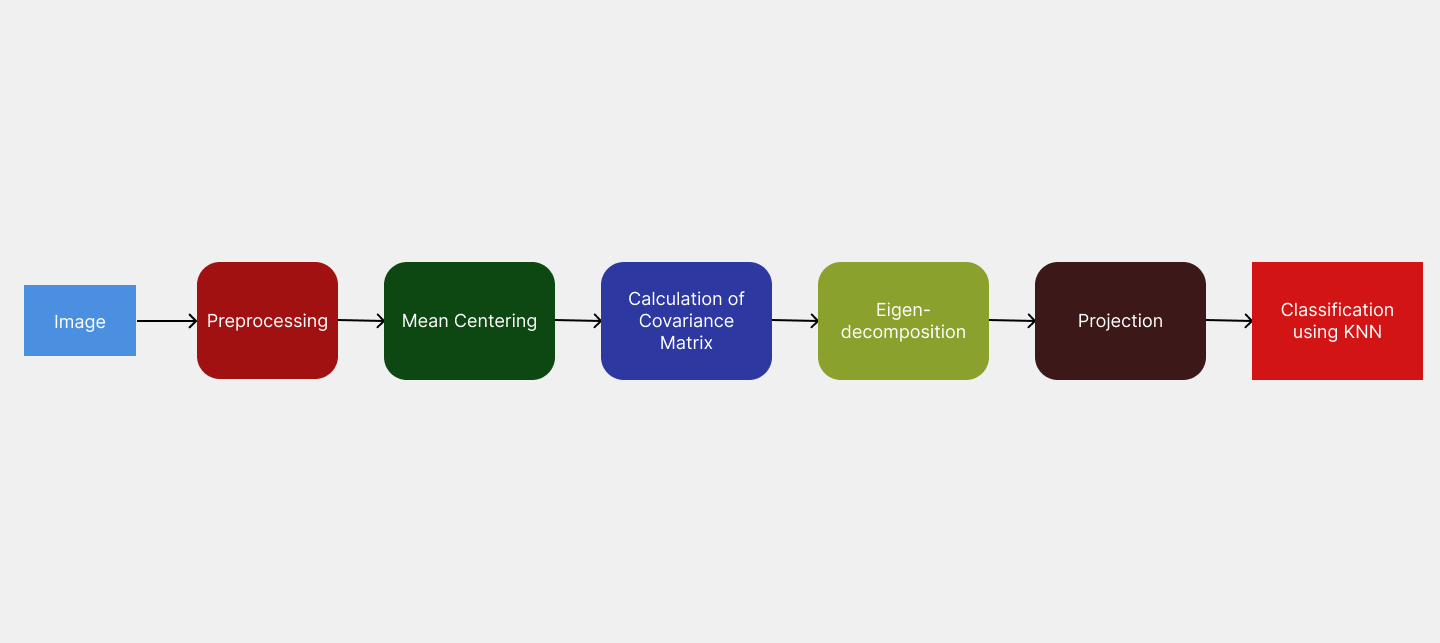
\includegraphics [width = 18cm, height = 7cm]  {PCA_workflow.png}}
        \caption{Workflow of the PCA approach }
    \end{figure}

    \begin{figure}[!hbt]
        \noindent\makebox[\textwidth]{%
        \includegraphics [width = 18cm, height = 6cm]  {Resnet-workflow.png}}
        \caption{Workflow of the ResNet-18 approach }
    \end{figure}
    
        \begin{figure}[!hbt]

   \subsection{Principal Component Analysis Approach}

    \begin{itemize}
        \item We followed each step exactly as explained in the theory.

        \item Even on the software implementation, we got an accuracy of meagre 72\%.

        \item Being in-eficient, this approach was discarded.
    \end{itemize}
        
    \begin{subfigure}{0.5\textwidth}
        \centering
        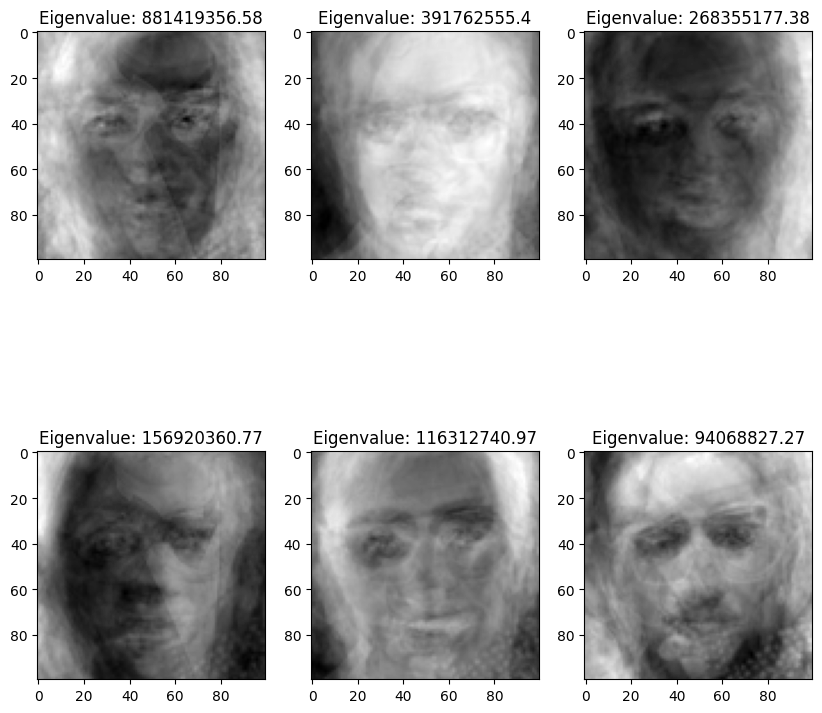
\includegraphics[height=6cm]{pca_eigenfaces.png}
        % \caption{Top 6 eigen-faces for the corresponding dataset obtained in the PCA approach.}
        \hspace{2em}
    \end{subfigure}
    \begin{subfigure}{0.5\textwidth}
        \centering
        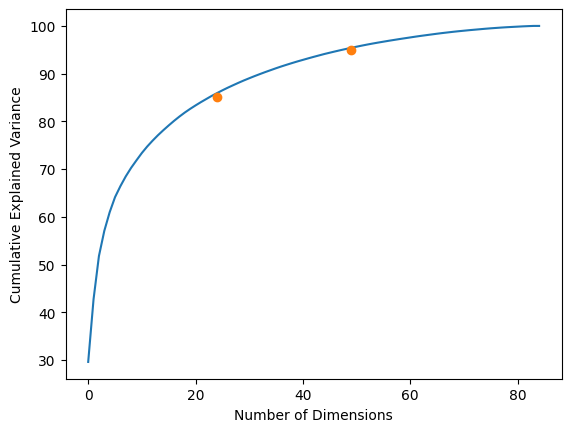
\includegraphics[height=6cm]{cum_ex_var.png}
        % \caption{Top 6 eigen-faces for the corresponding dataset obtained in the PCA approach.}
    \end{subfigure}
    
    \caption{Left:Top 6 Eigenfaces for the corresponding dataset and Right:Cumulative Explained Variance}
\end{figure}

 
    % \begin{figure}[!hbt]
    %     \noindent\makebox[\textwidth]{%
    %     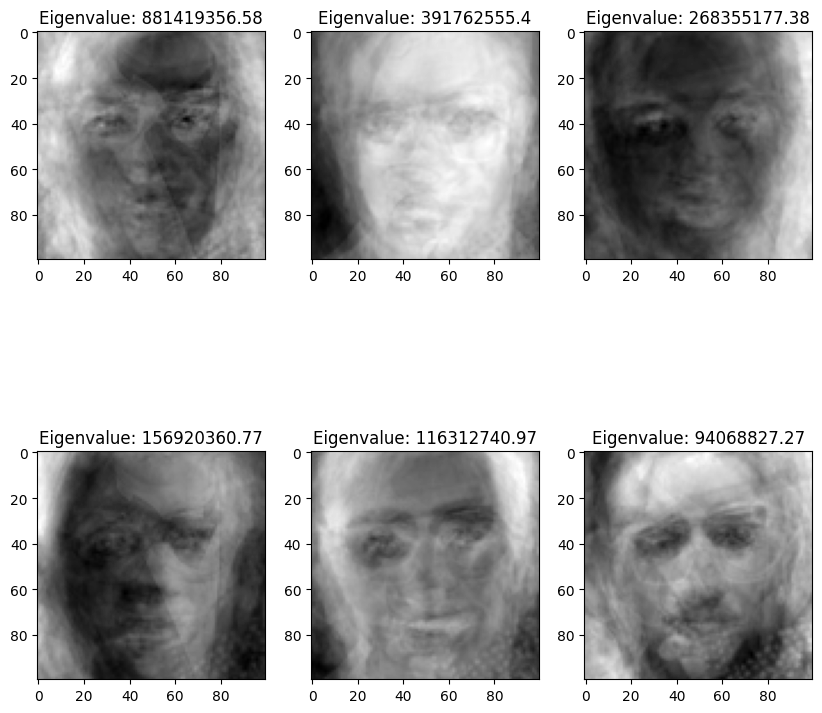
\includegraphics [height = 6cm]  {pca_eigenfaces.png}}
    %     \caption{Top 6 eigen-faces for the corresponding dataset obtained in the PCA approach.}
    % \end{figure}
    % \begin{figure}[!hbt]
    %     \noindent\makebox[\textwidth]{%
    %     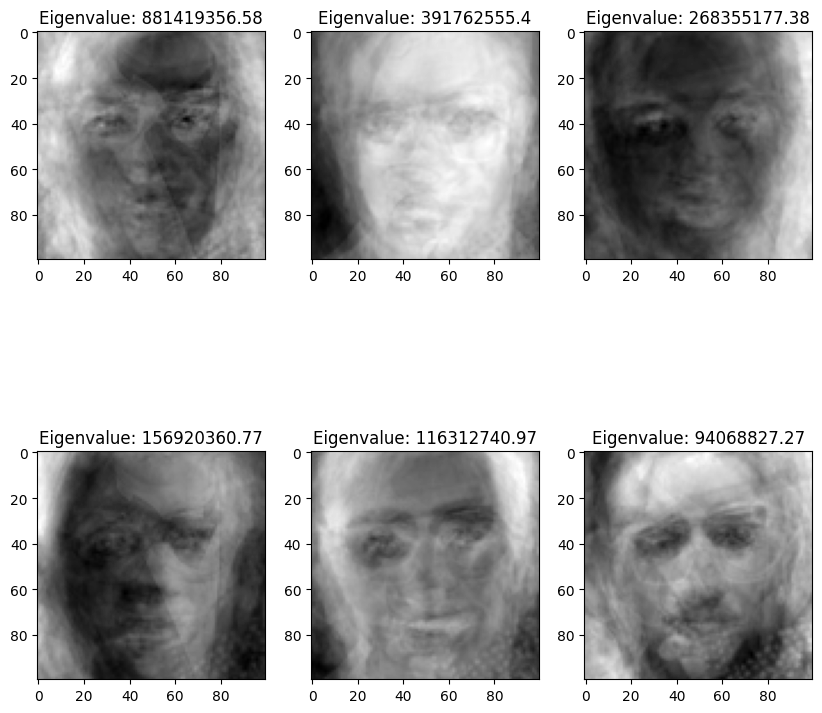
\includegraphics [height = 6cm]  {pca_eigenfaces.png}}
    %     \caption{Top 6 eigen-faces for the corresponding dataset obtained in the PCA approach.}
    % \end{figure}



    \newpage
    
    \subsection{ResNet-18 Approach}

    \begin{enumerate}
        \item \textbf{Resizing of the Images - }The obtained images were then resized to 224 x 224 pixels. This was done to ensure consistency in the data.

        \item \textbf{Data Augmentation - }For the next step, we employed geometric transformations as part of the data augmentation process. Geometric transformations involve altering the spatial properties of the images without changing their content, thereby diversifying the dataset and enhancing the model's ability to generalize across different facial variations.

        \begin{itemize}
            \item \textbf{Rotation - }We applied random rotation to face images within a specified range of angles. This allowed us to simulate variations in head orientation that may occur in real-world scenarios.
            By exposing the model to faces at different angles, we aimed to improve its ability to recognize and classify faces regardless of their orientation.

            \item \textbf{Translation - }Shifting the position of faces within the image was another geometric transformation we employed. This helped the model become invariant to slight changes in facial location.
            By randomly translating the faces horizontally and vertically, we introduced variability in facial position, making the model more robust to spatial shifts in real-world images.
            
        \end{itemize}

        The most prominent advantage of augmenting data is that it makes our model robust, and was one of the major reason that we discarded the Principal Component Analysis approach and shifted to a Convolutional Neural Network.
   \begin{figure}[!hbt]
                \noindent\makebox[\textwidth]{%
                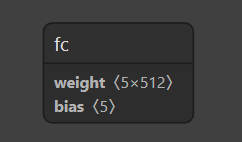
\includegraphics [ height = 2cm]  {model_fc.png}}
                \caption{Fully Connected Layer }
            \end{figure}
        \item \textbf{Modifications in the Fully Connected Layer and inference - }

        \begin{itemize}
            \item From the input image, we extracted the features and flattened them into a vector of dimension 1x512. This was the vector \textbf{X}.

            \item The weights of this layer are stored in the matrix \textbf{W}. Its dimensions are \textbf{512x5}.

            \item  The bias of the model is the vector \textbf{B}. Its dimensions are \textbf{1x5}.

            \item The weights of the next layer, i.e., the output layer are represented as \[Y = XW + B\]. The dimensions of Y are \textbf{1x5}.

            \item These 5 values denote the percentage similarity the input image has to the 5 celebrities we have trained our model on. It simply picks up the maximum of the those and classifies the image into that particular class. E.g. - if the vector is \[[2.0042446, -6.1100012,\textbf{ 96.5389821},  0.02223242, 1.024533324]\] the model would classify the image to class 3, which is \textbf{Jerry Seinfeld} in this case.

            \item We ran the training on \textbf{35 Epochs}, and got an accuracy of \textbf{96\%} on the testing data.

        \end{itemize}

\item \textbf{Feature and Weight Extraction}
\begin{itemize}
    \item \textbf{Feature Extraction after the avg pool layer was done via }
\end{itemize}

    \item \textbf{Validation and Performance Analysis}

To assess the effectiveness of our model, we employed two key validation techniques:

\begin{enumerate}
    \item \textbf{Confusion Matrix:} We visualized the performance of our model using a confusion matrix. This matrix provides a detailed breakdown of how the model classified the input data. Ideally, the diagonal elements of the confusion matrix should have high values, indicating accurate predictions for each class. Conversely, low values off the diagonal represent correct classifications assigned to the wrong class.
    \item \textbf{Loss Plot and Preventing Overfitting:} We monitored the model's loss function throughout the training process. The loss function quantifies the difference between the model's predictions and the actual ground truth. By plotting the loss function over epochs (training iterations), we can observe how the model's performance evolves. Typically, the loss function decreases as the model learns from the training data. However, if the loss starts to increase after a certain point, it could indicate overfitting.
    By analyzing the loss plot, we were able to determine the optimal number of epochs for training. In this case, 35 epochs were identified as the stopping point to avoid overfitting. Overfitting occurs when the model memorizes the training data too well, leading to poor performance on unseen data. By stopping the training process before overfitting sets in, we ensure the model generalizes well to new data.

\end{enumerate}
This combined approach, utilizing both the confusion matrix and the loss plot, provides a comprehensive understanding of the model's performance and helps us achieve optimal results.

\begin{figure}[!hbt]
    \begin{subfigure}{0.5\textwidth}
        \centering
        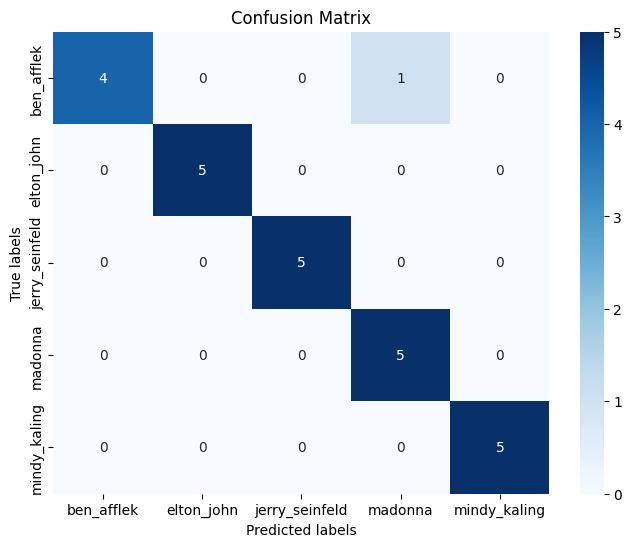
\includegraphics[height=6cm]{confusion_matrix.png}
        % \caption{Top 6 eigen-faces for the corresponding dataset obtained in the PCA approach.}
        \hspace{2em}
    \end{subfigure}
    \begin{subfigure}{0.5\textwidth}
        \centering
        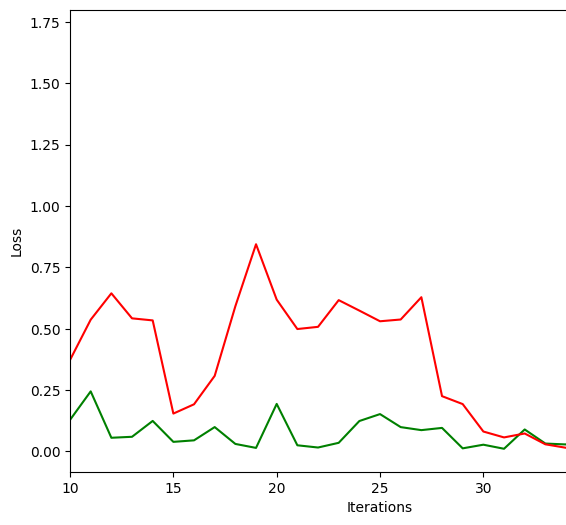
\includegraphics[height=6cm]{loss_epoch.png}
        % \caption{Top 6 eigen-faces for the corresponding dataset obtained in the PCA approach.}
    \end{subfigure}
    \caption{Left: Confusion Matrix || || Right: Loss vs Epochs - Red: Test Loss - Green: Train Loss}
\end{figure}
    
    \end{enumerate}
\section{Hardware Implementation}
  
        \subsection{FPGA hardware} 
All designs were targeted towards the Nexys A7-100T FPGA.
The Nexys A7-100T is a digital circuit development board from Digilent that uses an AMD Artix 7 field programmable gate array (FPGA). The board has the following features: Four Pmod ports 12-bit VGA output USB HID Host for mice, keyboards, and memory sticks Two 4-digit 7-segment displays Temperature sensor PDM microphone Two tri-color LEDs 16 user LEDs 16 user switches 3-axis accelerometer The Nexys A7 has 15,850 programmable logic slices, 4,860 Kbits of fast block RAM, 240 DSP slices, and six clock management tiles. It also has 128 MiB DDR2 SDRAM and 16 MiB serial Flash, 16 switches, two RGB LEDs, and a USB-UART bridge. The board can be powered by an external power supply or the USB-JTAG port. 

        \subsection{FPGA Building Blocks} 
\begin{enumerate}
        
           \item  \textbf{UART}
   
\begin{itemize}
    \item \textbf{Feature Extraction in Python:} We are using Python to preprocess the image and extract a feature vector of dimension 1x512 from it. Single-precision floating-point numbers (standard IEEE-754 format) are used to represent each feature unit.
    \item \textbf{Transfer via UART:}  UART interfaces have limitations on data size. They typically transmit data in 8-bit chunks (1 byte). Sending large floating-point values (4 bytes each) is done in 4 clock cycles. A different Serial transfer protocol can be implemented in the future to increase this speed.

\end{itemize}

\item \textbf{B-RAM}
We have initialized the weights and bias of the final fully connected layer in a B-RAM to decrease the transfer time and making overall processing fast. B-RAM offers faster access compared to external memory, like DDR, further improving the efficiency of the fully connected layer.
                
      
\item \textbf{ALU based on Standard IEEE-754 } 
                \\
                Here's a breakdown of the ALU:

\begin{itemize}
\item \textbf{IEEE-754 and Floating-Point Numbers:}

The IEEE-754 standard defines a format for representing floating-point numbers in binary format. These numbers consist of three parts:

\begin{itemize}
    \item \textbf{Sign bit:} Indicates positive or negative value.
    \item \textbf{Exponent:} Represents the magnitude of the number.
    \item \textbf{Mantissa (Significand):} Holds the fractional part of the number.
\end{itemize}
\item\textbf{ALU Operations:}
\begin{itemize}
    \item \textbf{Addition/Subtraction:}
\begin{itemize}
        \item The ALU aligns the exponents of the two operands (numbers) by shifting the mantissas if necessary.
        \item It performs addition or subtraction on the aligned mantissas.
        \item Finally, it adjusts the exponent and normalizes the result based on IEEE-754 rules.
\end{itemize}

    \item \textbf{Multiplication:}

\begin{itemize}
        \item The ALU multiplies the mantissas of the operands.
        \item It adds the exponents together.
        \item Again, it normalizes the result according to the IEEE-754 standard.
\end{itemize}

 
            \end{itemize}
          \end{itemize} 
           \item  \textbf{Fully Connected Layer: }
             We utilized FPGA's hardware for efficient matrix multiplication, a core operation in our model, while utilizing softmax for output selection in the final layer. Here's a breakdown of the key points:

\begin{itemize}
    \item \textbf{Pre-loaded Weights and Coefficients:} By storing the trained model's weights and coefficients directly in Block RAM (BRAM) on the FPGA, we significantly reduced processing time compared to calculating them during runtime.
    \item \textbf{Faster Memory Access:} BRAM offers faster access compared to external memory, like DDR, further improving the efficiency of the matrix multiplication layer.
     \item \textbf{Algorithm:}

The multiplication was done as follows - 
    \begin{enumerate}
        \item The weight matrix W can be represented as
        \[[W_1, W_2, W_3, W_{4}, W_{5}]\]

        \item Column j of the intermediate matrix is \[\sum_{i=1}^{512}{W_{ij}X_{i}}\].
    
        \item Instead of adding the values in place, we first store the values individually in a temporary matrix and then add them.
        \item Finally we add the bias matrix B to the obtained matrix in-place
    \end{enumerate}
Following the multiplication, the maximum of all the the 5 outputs is calculated and the corresponding LED is lit.
 \end{itemize}
\item \textbf{LED Controller}
 This module lights up the corresponding LED according to the Softmax output of the fully connected layer.
 \end{enumerate}
\subsection{Difficulties:}
\begin{enumerate}
    \item \textbf{UART Interface and Memory Storage:}
Implementing the UART interface and storing data efficiently in memory were critical aspects of the project.

    \item \textbf{Matrix Multiplication and Writer Pointer Logic:}
Defining a robust coding logic for the writer pointer during matrix multiplication proved challenging.

    \item \textbf{Latch Removal:}
Eliminating latches introduced during memory fetching required additional effort. This was addressed by:

\begin{itemize}
        \item Adding necessary \verb|else| statements.
        \item Replacing combinational logic with sequential logic in memory fetching sections.
\end{itemize}

    \item \textbf{Finite State Machine (FSM):}
Implementing an FSM facilitated the management of individual parts within each process, making the design more modular and easier to understand.
\end{enumerate}

\subsection{Optimizations for Synthesizable Code:}

\begin{enumerate}
    \item \textbf{Latch Detection and Elimination:}

\begin{itemize}
        \item The code was analyzed to identify unintended latches inferred by the compiler in combinational logic sections.
        \item To eliminate these latches:

    \begin{itemize}
            \item The inference report was used to pinpoint the specific combinational procedures and latch names.
            \item Variables were fully specified in all cases within the code.
    \end{itemize}

\end{itemize}

    \item \textbf{Case Statement Inference:}
The behavior of case statements was verified to ensure they were interpreted as intended (full/parallel case statements).

    \item \textbf{Incomplete Event List Warnings:}
Any warnings related to incomplete event lists were addressed to ensure proper event handling.

    \item \textbf{Unconnected Ports:}
The design schematic was reviewed to identify and connect any unused ports.

\end{enumerate}

 \newpage
\subsection{Schematics} 
        \begin{figure}[!hbt]
                \noindent\makebox[\textwidth]{%
                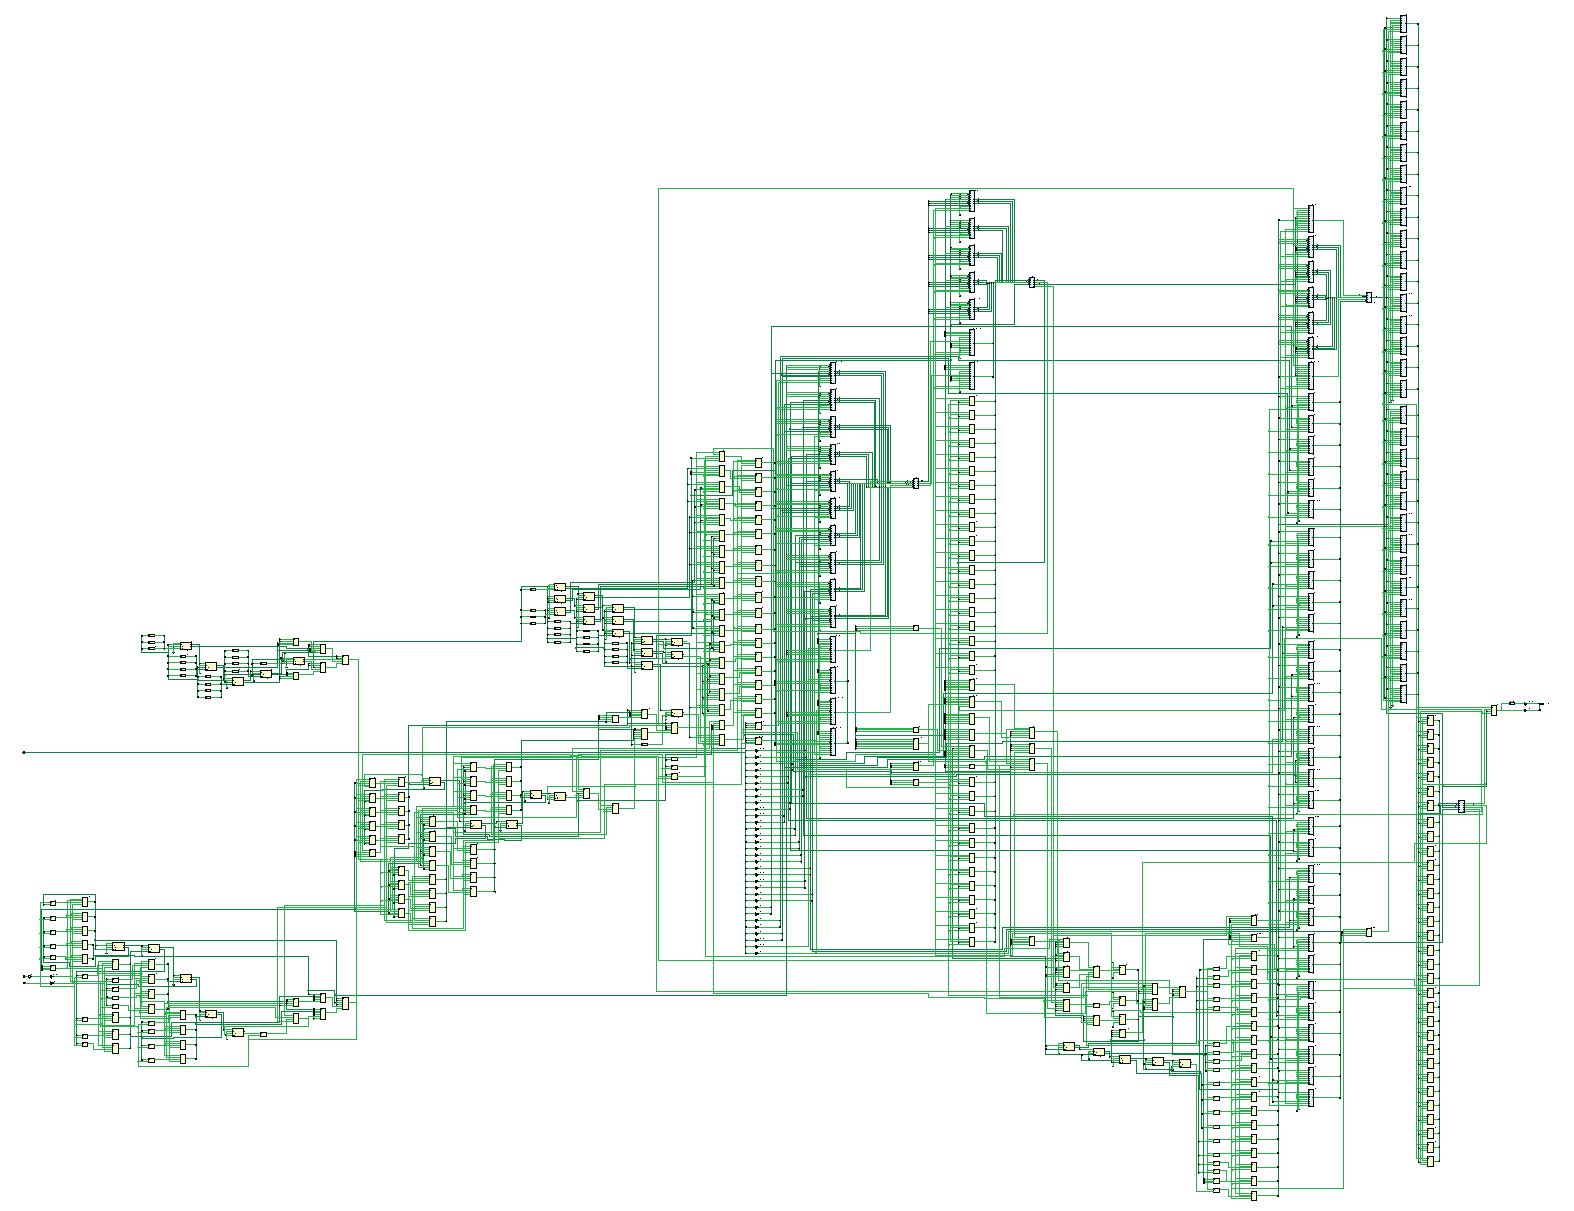
\includegraphics [width = 18cm, height = 7cm]  {fc_schematic.png}}
                \caption{Fully Connected Layer Schematic }
            \end{figure}
        \begin{figure}[!hbt]
        \noindent\makebox[\textwidth]{%
        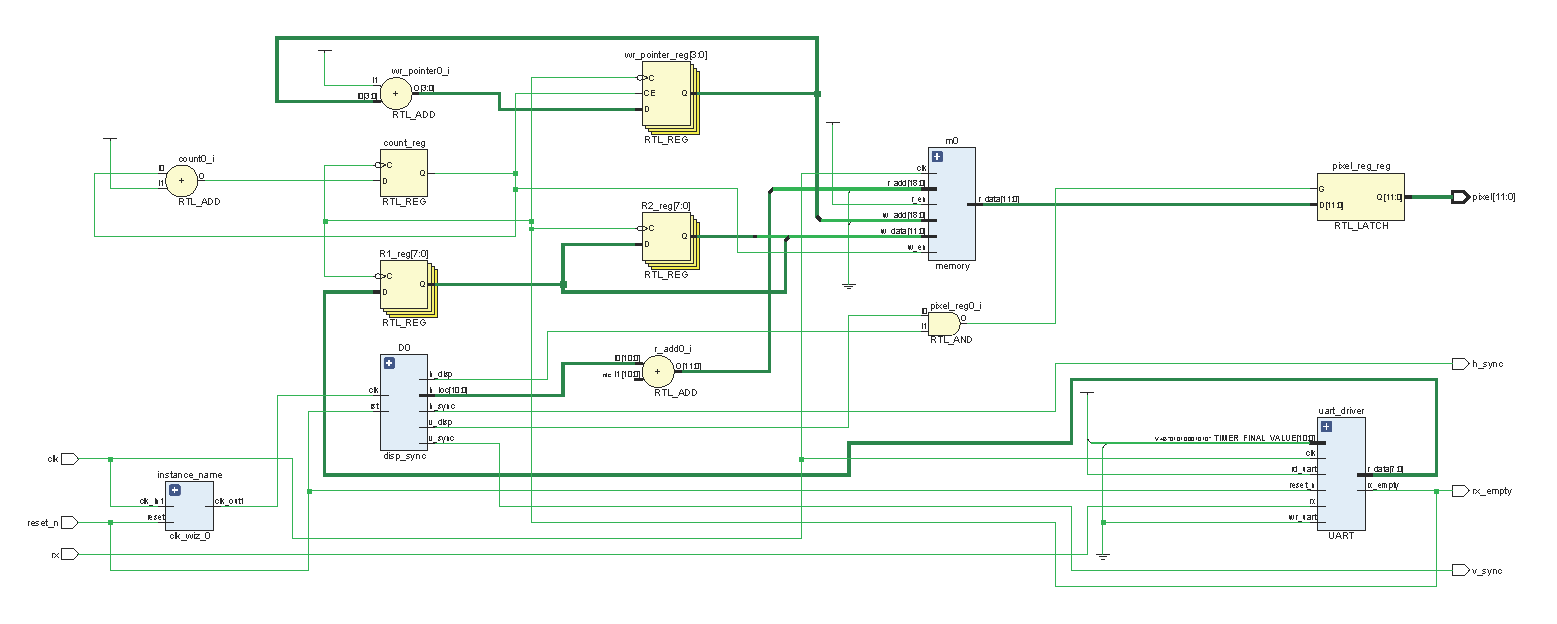
\includegraphics[width=18cm, height=7cm]{uart_schematic.png}}
        \caption{UART Schematic}
    \end{figure}
    


% \newpage
\section{Working and Results}

\begin{figure}[!hbt]
        \noindent\makebox[\textwidth]{%
        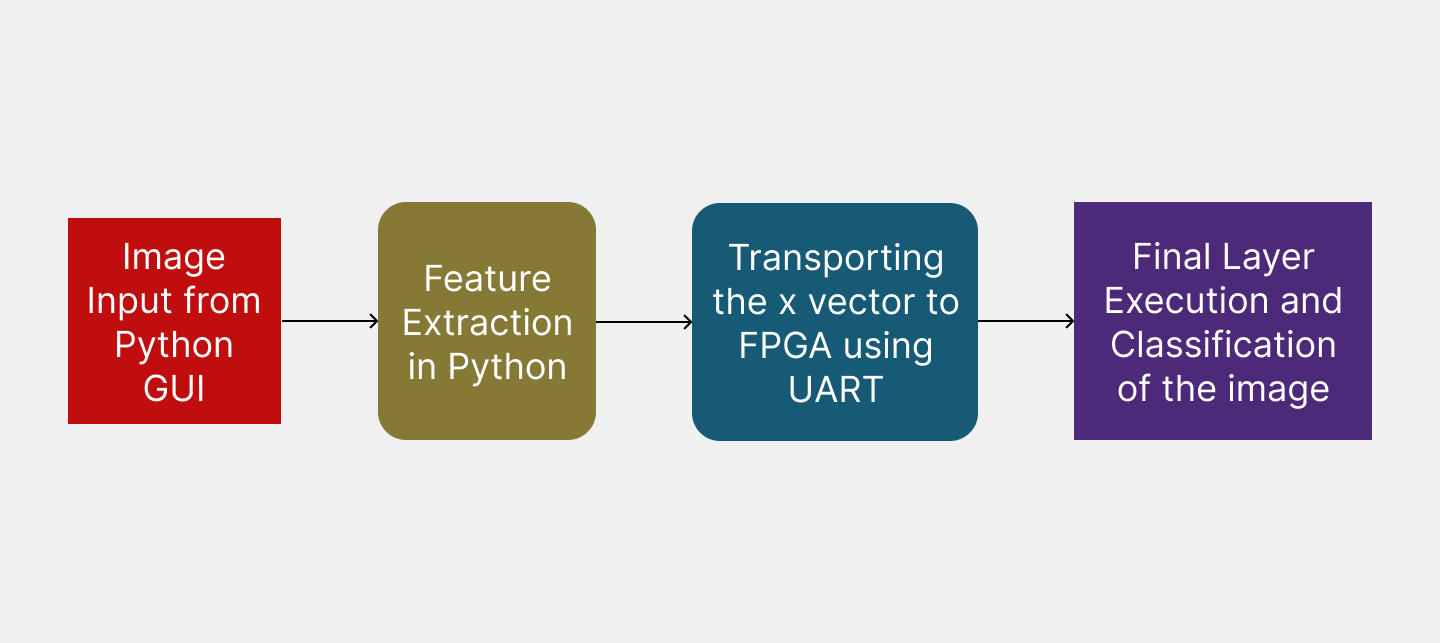
\includegraphics [width = 18cm]{pipeline.png}}
        \caption{Final Pipeline.}
\end{figure}

  \begin{figure}[!hbt]
        \noindent\makebox[\textwidth]{%
        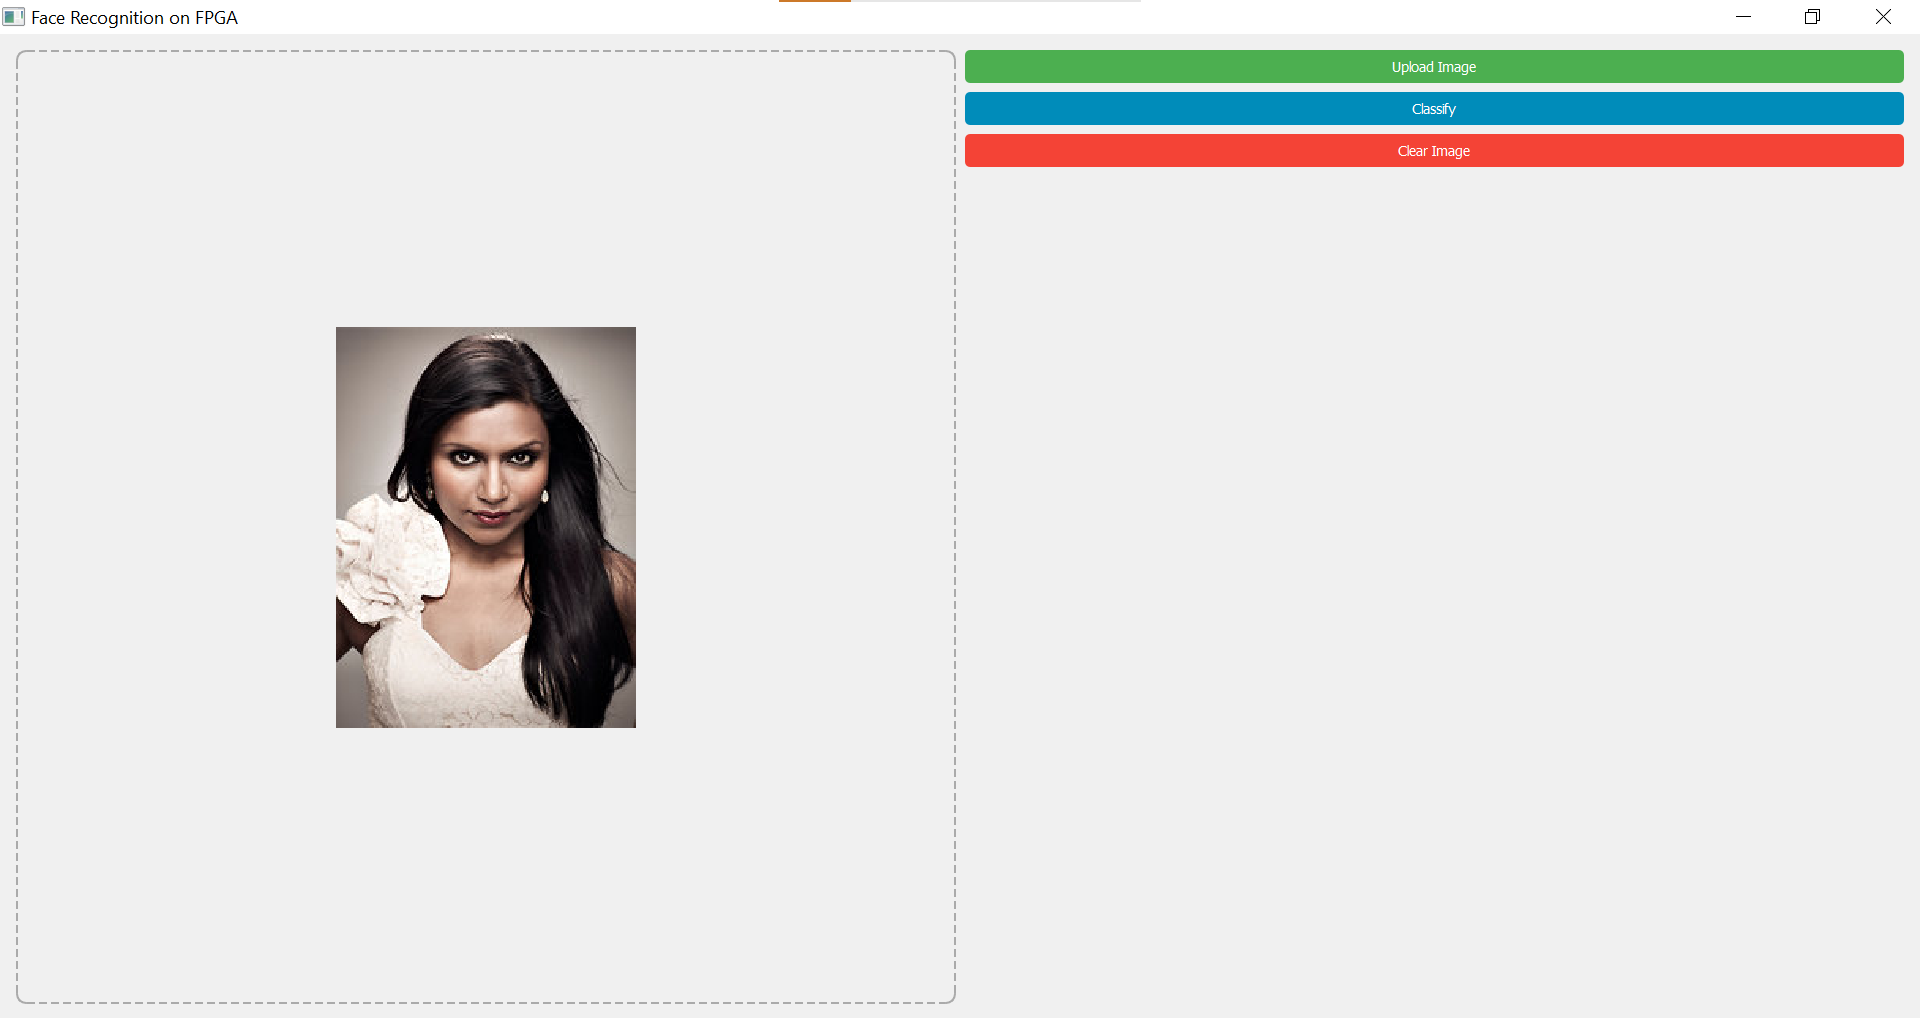
\includegraphics [width = 18cm]  {gui.png}}
        \caption{Graphical User Interface for Interacting with FPGA. }
    \end{figure}
    
    \begin{figure}[!hbt]
        \noindent\makebox[\textwidth]{%
        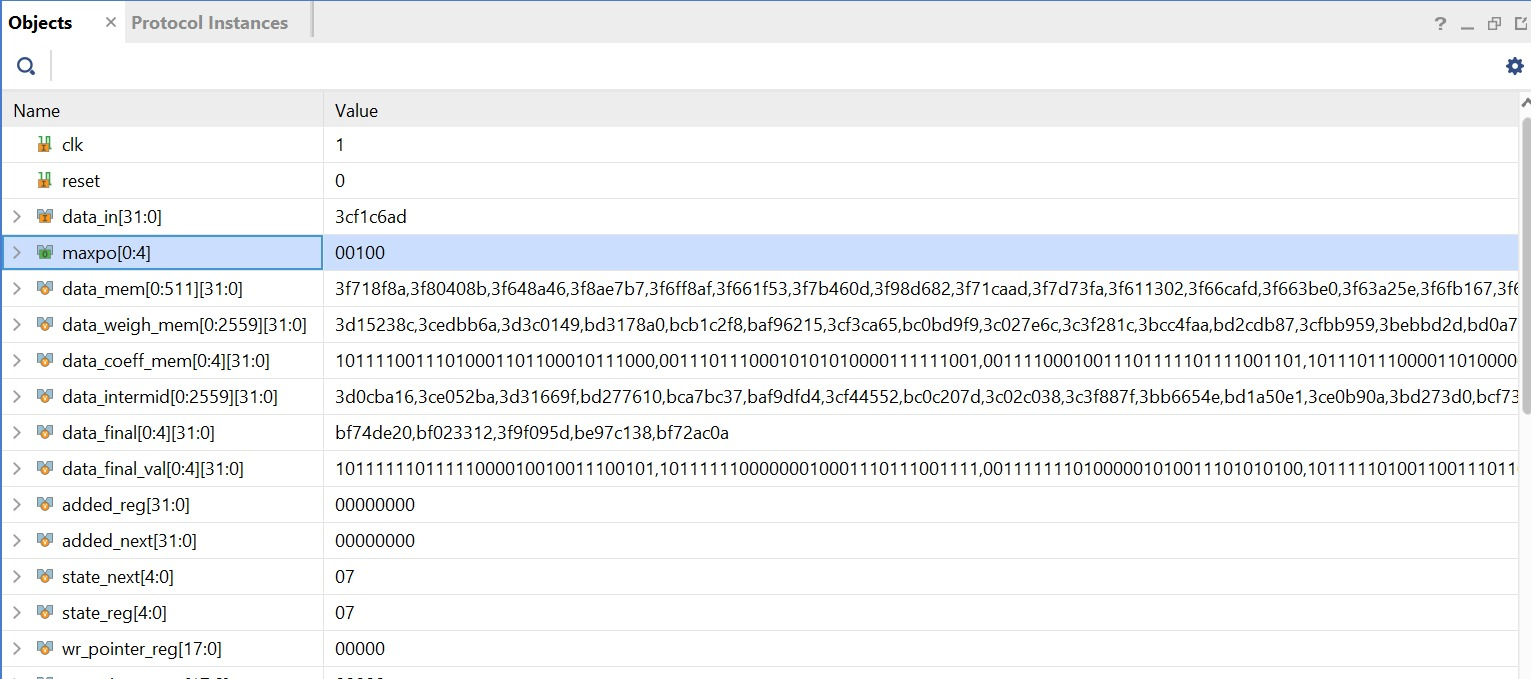
\includegraphics [width = 18cm, height = 7cm]  {Simulaton Results.jpg}}
        \caption{Output on simulation in Vivado.}
    \end{figure}
    
    \begin{figure}[!hbt]
        \noindent\makebox[\textwidth]{%
        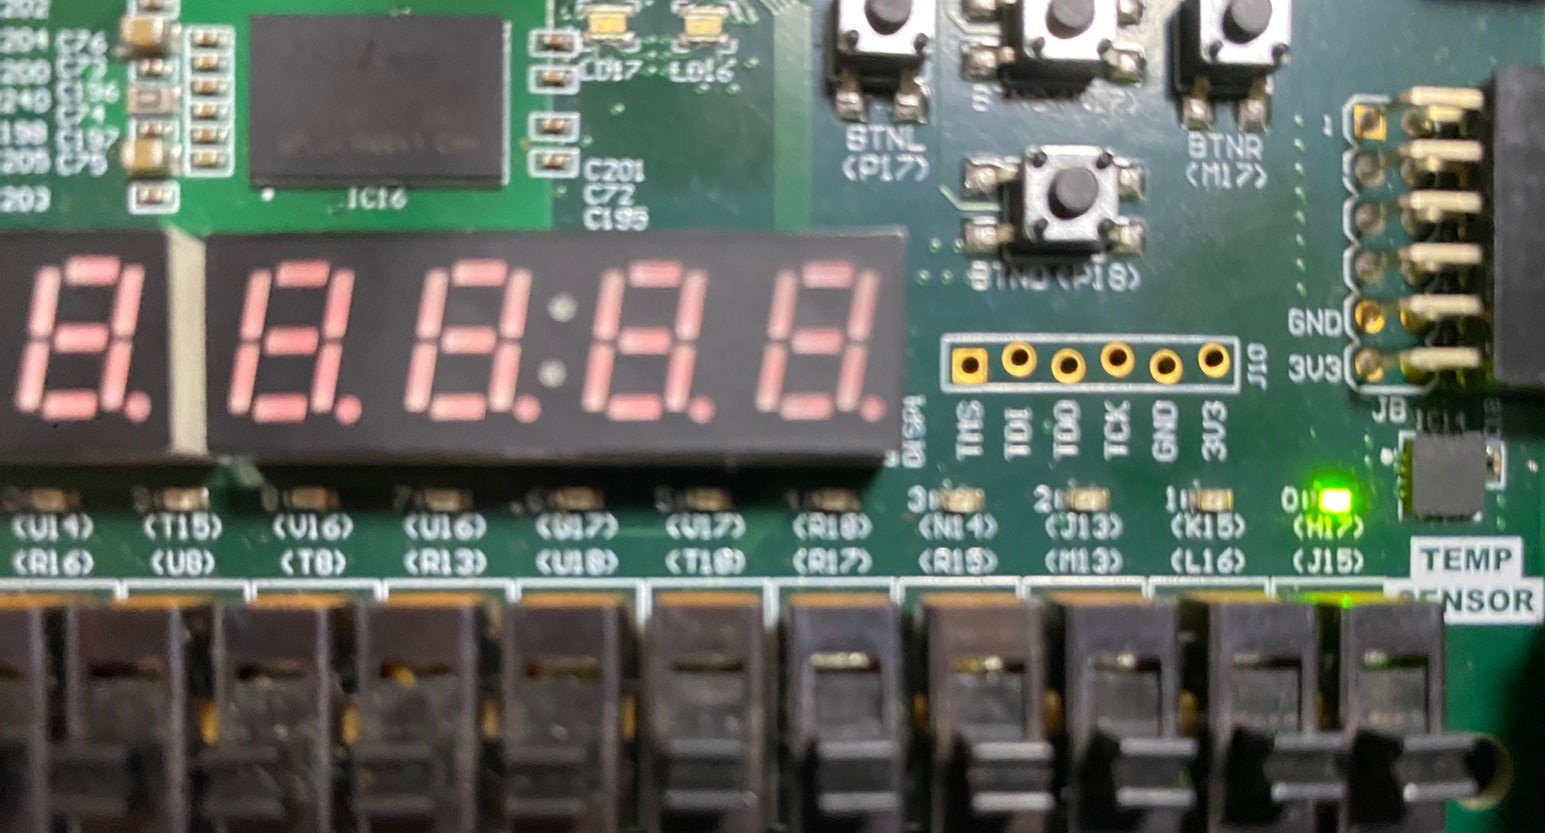
\includegraphics [width = 18cm, height = 7cm]  {fpga.jpg}}
        \caption{Output on FPGA || Indicating that class - 5 is classified.}
    \end{figure}

\begin{enumerate}
\item \textbf{Pipeline}
The final pipeline consists of the following steps.
\begin{itemize}
    \item Python GUI interface to interact with the FPGA.
    \item Preprocessing and feature extraction in python.
    \item Transporting the feature vector to FPGA via UART protocol.
    \item Execution of fully connected layer on FPGA and classification of the image
    \item Output displayed on the FPGA via LEDs and on python GUI.
\end{itemize}
\newpage

\item \textbf{Work-flow}
\begin{itemize}
\item We have integrated our model onto a Field Programmable Gate Array (FPGA) for facial recognition task. To provide a user-friendly interface for uploading images and displaying results, we developed a Python Graphical User Interface (GUI) [\textit{Fig 11}] using the PyQt5 module. This GUI allows users to upload an image from a laptop and displays it on the screen for visualization purposes.

\item Upon uploading an image, the Python GUI invokes a function responsible for extracting the features of the image. These features are then transmitted to the FPGA for further processing. The communication between the laptop and the FPGA is facilitated through a Universal asynchronous receiver-transmitter (UART) interface.

\item On the FPGA, the received features undergo inference using our trained face recognition model. The model performs classification directly on the FPGA board, enabling real-time processing without the need for external computing resources. To indicate the classification result, we have incorporated five Light Emitting Diodes (LEDs), each corresponding to a different facial class. Once the inference is complete, the LED corresponding to the class to which the input image belongs illuminates [\textit{Fig 11}], providing immediate feedback to the user.
\end{itemize}

\item \textbf{Resource Utilization}

\begin{itemize}
    \item The table in the \textit{Figure 13} shows how much hardware is available on the FPGA device (Available) and how much our design is using (Estimation). Each type of resource is listed (Resource), such as logic gates (LUTs), memory (LUTRAMs, FFs), and clock buffers (BUFGs). DSP slices are for signal processing (DSP).
    \item The number of FF used in the synthesis is same as intended by design, implying the code will be synthesisable.
     \begin{figure}[!hbt]
        \noindent\makebox[\textwidth]{%
        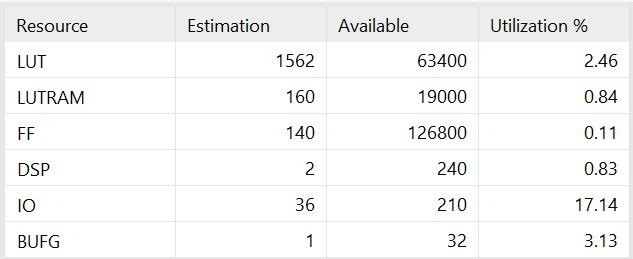
\includegraphics [width = 18cm, height = 7cm]  {Resource Utilization.jpg}}
        \caption{Total Resource Utilization }
    \end{figure}
\end{itemize}
    \item  \textbf{Timing Report}
    \begin{itemize}
\item The simulation time of the fully connected layer is 87 µs per Image.
\item However, the image transfer from computer to FPGA takes around 1.6 s due to the limitations of the UART protocol.
\end{itemize}
\end{enumerate}
\section{Future Goals}
        \begin{enumerate}
            \item \textbf{Transporting the Entire Model to FPGA: }We plan to optimize and deploy the entire machine learning model onto a Field-Programmable Gate Array (FPGA), eliminating the need for data preprocessing on Python.

            \item \textbf{Real-Time Inference with Camera Input: }We aim to enable real-time inference using camera input, facilitating applications such as object detection, recognition, and tracking in real-world environments and use it to solve real world problems, like developing an attendance system in a class where the number of students is very high.

            \item \textbf{Transitioning from UART to Ethernet or USB: }we aim to enhance the communication efficiency between the FPGA and Python by transitioning from the UART (Universal Asynchronous Receiver-Transmitter) protocol to more robust and high-speed alternatives such as Ethernet or USB (Universal Serial Bus). This transition promises increased data transfer rates, reduced latency, and improved reliability, thereby optimizing the interaction between the FPGA-based hardware and the Python software.
        \end{enumerate}
     \newpage
     \section{References}

    \begin{enumerate}
        \item \href{https://www.youtube.com/watch?v=Kt-78I-NUgY&list=PL-iIOnHwN7NXw01eBDR7wI8KzGK4mu8Sr&pp=iAQB}{ECE 3300 - Digital Circuit Design Using Verilog}

        \item \href{https://www.sutherland-hdl.com/papers/2006-SNUG-Boston_standard_gotchas_presentation.pdf}{Subtleties in the Verilog and SystemVerilog Standards That Every Engineer Should Know! - Stuart Sutherland and Don Milis}

        \item \href{https://people.ece.cornell.edu/land/courses/ece5760/Verilog/coding_and_synthesis_with_verilog.pdf}{Verilog Synthesis Methodology - Finbarr O’Regan}

        \item \href{https://arxiv.org/pdf/1512.03385.pdf}{Deep Residual Learning for Image Recognition}

        \item \href{https://www.geeksforgeeks.org/ieee-standard-754-floating-point-numbers/}{IEEE Standard 754 Floating Point Numbers - GeeksForGeeks}

        \item \href{https://github.com/opencv/opencv/tree/master/data/haarcascades}{Haarcascade GitHub Repository}
    \end{enumerate}


        
\end{document}